\chapter{Centralized and Decentralized Optimal Freeway Control via the Discrete Adjoint Method}
\label{chapter:adjoint}

In  this chapter, we propose a discrete adjoint approach to compute optimal ramp-metering stategies on road networks modeled by conservation laws.
Networks of one-dimensional conservation laws,
described by systems of nonlinear first-order hyperbolic \textit{partial
differential equations}~(PDEs), are an efficient framework for modeling
physical phenomena, such as freeway traffic evolution~\cite{garavello2006traffic,work2010traffic,frazzoli2002real} and supply
chains~\cite{Brunnermeier1999}. Similarly, PDE systems of balance laws are useful in modeling gas pipeline flow~\cite{Gugat2011Gas,Rothfarb1970Optimal} and water channels~\cite{Gugat2012Contamination,Rabbani2010}. Optimization
and  control of these networks is an active field of
research~\cite{Gugat2005,Bayen2006,Kotsialos2004}. More generally, numerous
techniques exist for the control of conservation laws, such as, for example,
backstepping~\cite{Coron2013,Glass2007}, Lyapunov-based methods~\cite{Coron2013}, and
optimal control methods~\cite{Blanchard2013,Keller2013,jacquet2006optimal}.
In particular, a common  approach is to compute the gradient of the cost functional via the \textit{adjoint method}~\cite{Giles2000Introduction,Jameson2000Aerodynamic,Raffard2008}.
Nevertheless, its implementation in the framework of nonlinear conservation laws presents several difficulties linked to the discontinuous  character of the solutions. In particular, the presence of shocks in the solutions requires a careful sensitivity analysis based on the use of shift-differentials and generalized tangent vectors, see~\cite{Bressan1997ShiftDifferentiability,Ulbrich2002Sensitivity,Ulbrich2003AdjointBased}.

Extensive study has also been conducted on the choice of method for effectively computing the gradient via the adjoint. In particular, the continuous adjoint
method~\cite{Jacquet2005,Gugat2005,Moin1994,Reuther1996} operates directly on
the PDE and a so-called adjoint PDE system, which when solved can be used to
obtain an explicit  expression of the gradient of the underlying optimization
problem. Conversely,  the discrete adjoint
method~\cite{Giles2000,Gugat2005,Kotsialos2004} first discretizes a
continuous-time PDE and then requires the solution of a set of linear
equations  to solve for the gradient. Finally, a third approach exists, which
uses  automatic differentiation techniques to automatically generate an
adjoint  solver from the numerical representation of the forward
system~\cite{Muller2005,Giering1998}.

It is well known that the numerical treatment of the adjoint method imposes a careful choice of the discretization scheme to avoid the introduction of numerical errors  at discontinuities~\cite{Giles2003Discrete}.
Rigorous convergence results for optimization problems have been provided for Lax-Friedichs type schemes~\cite{Giles2010Convergencea} and relaxation methods~\cite{Banda2012Adjoint}.
The case of road networks in free flow conditions is addressed in~\cite{Gugat2005}.
In our more general setting of PDE networks and applications to freeway traffic control, the presence of junction conditions with both forward and backward-moving shockwaves led us the use of a modified Godunov scheme that precisely takes into account the flows at the network nodes. An alternative approach involves using Lax-Friedichs-type discretizations with higher-resolution interpolation schemes~\cite{Nessyahu1990NonOscillatory}. Moreover, general existence and stability results for the corresponding system of equations modeling traffic evolution on the network are still missing at the moment.
Therefore, establishing rigorous convergence results for the gradient computation in this framework is out of the scope of this thesis. Here we made the choice of the discrete adjoint approach, which derives the gradient directly from the discretized system, thus avoiding dealing with weak boundary conditions in the continuous system~\cite{garavello2006traffic,work2010traffic,strub2006weak}.

% we could use a variant of the lax-friedrichs.
% goettlich, staggered lax-friedrichs, to have a more precise approximation, lax friedrichs is very diffusive.





%While the continuous adjoint formulation results in a compact formulation, 
%better intuition into the system's sensitivities with respect to the objective, 
%and well-posedness of the control's solution (when it can be proved), it is 
%often difficult to derive for systems of hyperbolic nonlinear PDEs controlled 
%by boundary conditions, when these boundary conditions have to be written in the 
%weak sense.
%Additionally, the continuous adjoint must eventually be discretized in order to 
%produce numerical solutions for the optimization problem. Finally, the 
%differentiation of the forward PDE is sometimes problematic due to the lack of 
%regularity of the solution~\cite{garavello2006traffic,work2010traffic} which 
%makes the formal definition of the adjoint problem more difficult.
%The discrete adjoint approach derives the gradient directly from the 
%discretized system, thus avoiding working directly with weak boundary 
%conditions in the continuous 
%system~\cite{garavello2006traffic,work2010traffic,strub2006weak}.
%Automatic differentiation techniques can simplify the repetitive 
%steps of the discrete adjoint derivation, but sometimes at the cost of 
%sub-optimal code implementations with respect to memory and CPU 
%consumption~\cite{Giles}. A more-detailed analysis of the trade-offs associated 
%with each method is given in~\cite{Giles}.

There exist many applications of the adjoint method for control, optimization 
and estimation of physical systems in engineering. Shape optimization of 
aircraft~\cite{Reuther1996,Giles1997,Moin1994} has applied the method 
effectively to reduce the computational cost in gradient methods associated 
with the large number of optimization parameters. The technique has also been 
applied in parameter identification of biological systems~\cite{Raffard2008}. 
State estimation problems can be phrased as optimal control problems by setting 
the unknown state variables as control parameters and penalizing errors in 
resulting state predictions from known values. This approach has been applied 
to such problems as open water state estimation~\cite{Castaings2006,Strub2009} 
and freeway traffic state estimation~\cite{Jacqueta}.

Since conservation laws may be nonlinear by nature and lead to non-convex or 
nonlinear formulations of the corresponding optimization problem, fewer 
efficient optimization techniques exist for the 
discretized version of these problems than for convex problems for example. One 
approach is to approximate the system with a ``relaxed'' version in order to 
use efficient linear programming techniques. In transportation, by 
relaxing the Godunov discretization scheme, the linearization approach was used 
in~\cite{gomes2006optimal} for optimal ramp metering, and 
in~\cite{ziliaskopoulos2000linear} for optimal route assignment which is exact 
when the relaxation gap can be shown to be zero. The ramp 
metering technique in~\cite{Muralidharana} uses an additional control parameter 
(variable speed limits) to mimic the linearized freeway dynamics. While the 
upside of these methods is reduced computational complexity and the guarantee 
of finding a globally optimal solution, the downside is that the model of the 
linearized physical system may greatly differ from the actual system to which 
the control policies would be applied.

Another approach avoids discretization of the continuous system by taking advantage of certain simplifying assumptions in the dynamics. In~\cite{Fugenschuh2006Combinatorial}, the problem of finding optimal split ratios on a traffic networks is efficiently solved by deriving non-linear and linear algebraic formulations of a simplified form of the continuous system dynamics which only considers forward-moving shockwaves. In~\cite{Apice2010Modeling}, a mixed-integer linear program (MILP) formulation is posed for the optimal routing of goods on a supply chain, leading to efficient solutions of this particular application. The number of integer constraints needed in the MILP formulation is proportional to the number of non-linear constraints in the underlying system and has a direct impact on the efficiency of MILP solvers. Applications to highly non-linear systems such as freeway traffic may prefer non-linear programming approaches such as the adjoint method using non-linear discretization techniques, which avoid integer constraints and allow the constraints to capture more complex dynamics.

Alternatively, nonlinear optimization techniques can be applied to the 
discretized system without any modification to the underlying dynamics. This 
approach leads to more expensive optimization algorithms, such as gradient 
descent, and no guarantee of finding a global optimum. One difficulty in this 
approach comes in the computation of the gradient, which, if using finite 
differences, requires a full forward-simulation for each perturbation of a 
control parameter. This approach is taken in~\cite{Ramon2013,Frejo2011} to 
compute several types of decentralized ramp metering strategies. The increased 
complexity of the finite differences approach for each additional control 
parameter makes the method unsuitable for real-time application on 
moderately-sized freeway networks.

Ramp metering is a common freeway control strategy, providing a means of 
dynamically controlling freeway throughput without directly impeding mainline 
flow or implementing complex tolling systems. While metering strategies have 
been developed using microscopic models~\cite{Ben-Akiva2003}, most strategies 
are based off macroscopic state parameters, such as vehicle density and the 
density's relation to 
speed~\cite{richards1956shock,lighthill1955kinematic,daganzo1995cell}. Reactive 
metering strategies~\cite{Papageorgiou1991Alinea,Papamichail,Kachroo2003} use 
feedback from freeway loop detectors to target a desired mainline density, 
while predictive metering 
strategies~\cite{Frejo2011,Kotsialos2004,gomes2006optimal,Chen1997} use a 
physical model with predicted boundary flow data to generate policies over a 
finite time horizon. Predictive methods are often embedded within a model 
predictive control loop to handle uncertainties in the boundary data and 
cumulative model errors~\cite{Muralidharana}.

This section develops a framework for efficient control of discretized 
conservation law PDE networks using the adjoint 
method~\cite{Giles2000,Pironneau1974} via Godunov 
discretization~\cite{godunov1959}, while detailing its application to 
coordinated ramp metering on freeway networks. Note that the method can be 
extended without significant difficulty to other numerical schemes commonly 
used to discretize hyperbolic PDEs. We show how the complexity of 
the gradient computation in nonlinear optimal control problems can be greatly 
decreased by using the discrete adjoint method and exploiting the decoupling 
nature of the problem's network structure, leading to efficient gradient 
computation methods. After giving a general framework for computing the gradient 
over the class of scalar conservation law networks, we show that the system's 
partial derivatives have a sparsity structure resulting in gradient computation 
times linear in the number of state and control variables for networks of small 
vertex degree. Memory usage is also linear when sparse data structures are utilized. The results are 
demonstrated by running a coordinated ramp metering strategy on a 19 mile 
freeway stretch in California faster than real-time, while giving traffic 
performance superior to that of state of the art practitioners tools.

% \todo{this is incorrect, make the overview match}
% The rest of the article is organized as follows. 
% Section~\ref{sec:Preliminaries} gives an 
% overview of scalar conservation law networks and their discretization via the 
% Godunov method, while introducing the nonlinear, finite-horizon optimal control 
% problem. Section~\ref{sec:Adjoint-method} details the adjoint method derivation 
% for this class of problems and shows how it can be used to compute the gradient 
% in linear time in the number of discrete state and control variables.  
% Section~\ref{sec:Applications-to-Optimal} shows how the adjoint method can be 
% applied to the problem of optimal coordinated ramp metering, with numerical 
% results on a real freeway network in California shown in 
% Section~\ref{sec:Numerical-results-for}. Finally, some concluding remarks are 
% given in Section~\ref{sec:Conclusions}.


\section{Discrete Adjoint Derivation for Networked Conservation Laws}

Section~\ref{sec:preliminaries} developed a method for discretizing networked, scalar conservation laws. Once a Riemann solver is selected for the junction behavior, the matter of discretization via Godunov's method becomes routine. This section uses Godunov's method to construct an efficient and general method for gradient computations of control objectives constrained by networked conservation law systems.

\subsection{State, Control, and Governing Equations\label{sec:State,-control,-and}}

We now focus on controlling systems of the form
in Equation~\eqref{eq:composed-flux} in which some parts of the state
can be controlled directly (for example, in the form of boundary control).
We wish to solve the system in Equation~\eqref{eq:composed-flux} $T$
time-steps forward, i.e. we wish to determine the discrete state values
$\discrete{\link}{\tind}$ for all links $\link\in\links$ and all
time-steps $\tind\in\intrange 0{\ntime-1}$. Furthermore, at each
time-step $\tind$, we assume a set of ``control'' variables $\tuple{\condiscrete 1{\tind}}{\condiscrete{\ncontrols}{\tind}}\in\mathbb{R}^{\ncontrols}$
that influence the solution of the Riemann problems at junctions,
where $\ncontrols$ is the number of controlled values at each time-step,
and each control may be updated at each time-step. We assume that
a control may only influence a subset of junctions, which is a reasonable
assumption if the controls have some spatial locality. Thus, for a
junction $\jn\in\jns$, we assume without loss of generality that
a subset of the control parameters $\tuple{\condiscrete{\cind_{\jn}^{1}}{\tind}}{\condiscrete{\cind_{\jn}^{\ncontrols_{\jn}}}{\tind}}\in\mathbb{R}^{\ncontrols_{\jn}}$
influence the solution of the Riemann solver. Similar to the notation
developed for state variables, for control variables, we define $\junccon{\jn}{\tind}\defeq\tuple{\condiscrete{\cind_{\jn}^{1}}{\tind}}{\condiscrete{\cind_{\jn}^{\ncontrols_{\jn}}}{\tind}}$
as the concatenation of the control variables around the junction
$\jn$. To account for the addition of controls, we modify the Riemann
problem at a junction $\jn\in\jns$ at time-step $\tind$ to be a
function of the current state of connecting links $\juncstate{\jn}{\tind}$,
and the current control parameters $\junccon{\jn}{\tind}$. Then using
the same notation as before, we express the Riemann solver as:

\begin{eqnarray*}
	\RS_{\jn}: & \mathbb{R}^{\ninc_{\jn}+\nout_{\jn}}\times\mathbb{R}^{\ncontrols_{\jn}} & \rightarrow\mathbb{R}^{\ninc_{\jn}+\nout_{\jn}}\\
	& \left(\juncstate{\jn}{\tind},\junccon{\jn}{\tind}\right) & \mapsto\RS_{\jn}\left(\juncstate{\jn}{\tind},\junccon{\jn}{\tind}\right)=\junctrace{\jn}{\tind}.
\end{eqnarray*}


We represent the entire state of the solved system with the vector
$\state\in\mathbb{R}^{\nlinks\ntime}$, where for $\link\in\links$
and $k\in\intrange 0{\ntime-1}$, we have $\state_{\nlinks k+\link}=\discrete{\link}{\tind}$.
Similarly, we represent the entire control vector by $\control\in\mathbb{R}^{\ncontrols\ntime}$,
where $\control_{\ncontrols\tind+\cind}=\condiscrete{\cind}{\tind}$.

For each state variable $\discrete{\link}{\tind}$, write the corresponding
update equation $\syseq_{\link}^{\tind}$:

\begin{eqnarray*}
	\syseq_{\link}^{\tind}: & \mathbb{R}^{\nlinks\ntime}\times\mathbb{R}^{\ncontrols\ntime} & \rightarrow\mathbb{R}\\
	& \left(\state,\control\right) & \mapsto\syseq_{\link}^{\tind}\left(\state,\control\right)=0.
\end{eqnarray*}
This takes the following form:

\begin{eqnarray}
	h_{\link}^{0}\left(\state,\control\right)=\discrete{\link}0-\initdiscrete_{\link} & =0\label{eq:init-ge}\\
	\syseq_{\link}^{\tind}\left(\state,\control\right)=\discrete{\link}{\tind}-\discrete{\link}{\tind-1}+\frac{\Delta t}{L_{\link}}f\left(\RS_{\jdown{\link}}\left(\juncstate{\jdown{\link}}{\tind-1},\junccon{\jdown{\link}}{\tind-1}\right)\right)_{\link}\nonumber \\
	-\frac{\Delta t}{L_{\link}}f\left(\RS_{\jup{\link}}\left(\juncstate{\jup{\link}}{\tind-1},\junccon{\jup{\link}}{\tind-1}\right)\right)_{\link} & =0 & \forall k\in\intrange 2{\ntime-1},\label{eq:main-ge}
\end{eqnarray}
or in terms of the Godunov junction flux:

\begin{eqnarray}
	\syseq_{\link}^{\tind}\left(\state,\control\right)= & \discrete{\link}{\tind}-\discrete{\link}{\tind-1} & +\dfrac{\Delta t}{\Delta x}\left(\god_{\jdown{\link}}\left(\juncstate{\jdown{\link}}{\tind},\junccon{\jdown{\link}}{\tind-1}\right)\right)_{\link}\nonumber \\
	&  & -\dfrac{\Delta t}{\Delta x}\left(\god_{\jup{\link}}\left(\juncstate{\jup{\link}}{\tind},\junccon{\jup{\link}}{\tind-1}\right)\right)_{\link}\label{eq:syseq-god}
\end{eqnarray}
for all links $\link\in\links$, where $\initdiscrete_{\link}$ is
the initial condition for link $\link$. Thus, we can construct a
system of $\nlinks T$ governing equations $H\left(\state,\control\right)=0$,
where the $h_{\link,k}$ is the equation in $H$ at index $\nlinks k+\link$,
identical to the ordering of the corresponding discrete state variable.

\paragraph{Optimal Control Problem Formulation\label{par:Optimization-Problem}}

In addition to our governing equations $\sys\left(\state,\control\right)=0$, where we assume each $h_i^k \in \mathcal{C}^1$,
we also introduce a cost function $\cost \in \mathcal{C}^1$.

\begin{eqnarray*}
\cost: & \mathbb{R}^{\nlinks T}\times\mathbb{R}^{\ncontrols T} & \rightarrow\mathbb{R}\\
& \left(\state,\control\right) & \mapsto\cost\left(\state,\control\right)
\end{eqnarray*}
which returns a scalar that serves as a metric of performance of the
state and control values of the system. We wish to minimize the quantity
$\cost$ over the set of control parameters $\control$, while constraining
the state of the system to satisfy the governing equations $\sys\left(\state,\control\right)=0$,
which is, again, the concatenated version of~\eqref{eq:main-ge} or~\eqref{eq:syseq-god}.
We summarize this with the following optimization problem:

\begin{eqnarray}
\underset{\control}{\min} & \cost\left(\state,\control\right)\nonumber \\
\text{subject to:} & \sys\left(\state,\control\right)=0\label{eq:op-problem}
\end{eqnarray}
Both the cost function and governing equations may be non-convex in
this problem.

% \subsection{Discrete Adjoint Overview}

% \subsection{Application to Networked Conservation Laws}
\subsection{Discrete Adjoint Method}
\label{sec:discrete-adjoint-method}

We wish to use gradient information in order to find control values
$\control^{*}$ that give locally optimal costs $\cost^{*}=\cost\left(\state\left(\control^{*}\right),\control^{*}\right)$.
Since there may exist many local minima for this optimization problem~\eqref{eq:op-problem}
(which is non-convex in general), gradient\emph{ }methods do not guarantee
global optimality of $\control^{*}$\emph{. }Still, nonlinear optimization
methods such as interior point optimization utilize gradient information
to improve performance~\cite{Andreas2005}.

In a descent algorithm, the optimization procedure will have to descend
a cost function, by coupling the gradient, which, at a nominal point
$\left(\nominal{\state},\nominal{\control}\right)$ is given by:

\begin{equation}
d_{\control}\cost\left(\nominal{\state},\nominal{\control}\right)=\evaluate{\pfrac{\cost\text{\ensuremath{\left(\state,\control\right)}}}{\state}}{\nominal{\state},\nominal{\control}}\Dfrac{\state}{\control}+\evaluate{\pfrac{\cost\text{\ensuremath{\left(\state,\control\right)}}}{\control}}{\nominal{\state},\nominal{\control}}\label{eq:j-v}.
\end{equation}

\begin{note}
For Equation~\eqref{eq:j-v} to be valid, all required partial and full derivatives must be well-defined, including $\Dfrac{\state}{\control}$. In some applications, this assumption does not necessarily hold,
either because $f$ itself is not smooth or because $\god$ is not
smooth (and thus $H \notin \mathcal{C}^1$), as is the case for the LWR equation with concave fundamental diagrams. There are several settings in which the
conditions for differentiability are satisfied, see in particular~\cite{Gugat2005,Flasskamp2012}.
\end{note}

The main difficulty is to compute the term $\Dfrac{\state}{\control}$.
We take advantage of the fact that the derivative of $H\left(\state,\control\right)$
with respect to $\control$ is equal to zero along trajectories of
the system:

\begin{equation}
d_{\control}\sys\left(\nominal{\state},\nominal{\control}\right)=\evaluate{\pfrac{\sys\text{\ensuremath{\left(\state,\control\right)}}}{\state}}{\nominal{\state},\nominal{\control}}\Dfrac{\state}{\control}+\evaluate{\pfrac{\sys\text{\ensuremath{\left(\state,\control\right)}}}{\control}}{\nominal{\state},\nominal{\control}}=0\label{eq:h-v}.
\end{equation}


The partial derivative terms, $\Hx\in\mathbb{R}^{\nlinks\ntime\times\nlinks\ntime}$,
$\Hu\in\mathbb{R}^{\nlinks\ntime\times\ncontrols\ntime}$, $\Jx\in\mathbb{R}^{\nlinks\ntime}$,
and $\Ju\in\mathbb{R}^{\ncontrols\ntime}$, can all be evaluated (more
details provided in Section~\ref{sub:Evaluating--and}) and then
treated as constant matrices. Thus, in order to evaluate $d_{\control}\cost\left(\nominal{\state},\nominal{\control}\right)\in\mathbb{R}^{\ncontrols\ntime}$,
we must solve a coupled system of matrix equations.

\paragraph{Forward system.\label{par:Forward-system}}

If we solve for $\Dfrac{\state}{\control}\in\mathbb{R}^{\nlinks\ntime\times\ncontrols\ntime}$
in~\eqref{eq:h-v}, which we call the \emph{forward system}:

\[
\Hx\Dfrac{\state}{\control}=-\Hu,
\]
then we can substitute the solved value for $\Dfrac{\state}{\control}$
into~\eqref{eq:j-v} to obtain the full expression for the gradient.
Section~\ref{sub:Evaluating--and} below gives details on the invertibility
of $\Hx$, guaranteeing a solution for $\Dfrac{\state}{\control}$.


\paragraph{Adjoint system.\label{par:Adjoint-system}}

Instead of evaluating $\Dfrac{\state}{\control}$ directly, the adjoint
method solves the following system, called the adjoint system,
for a new unknown variable $\lambda\in\mathbb{R}^{\nlinks\ntime}$
(called the adjoint variable):

\begin{equation}
\Hx^{T}\lambda=-\Jx^{T}\label{eq:adjoint}
\end{equation}

Under certain additional conditions on the flux function and discretization scheme, the adjoint system in Equation~\eqref{eq:adjoint} may be shown to converge to the continuous adjoint system as the discretization steps go towards zero, as described in the following works~\cite{Banda2012Adjoint,Gugat2005,ulbrich2003adjoint}. No such convergence results exist in our setting of using a Godunov discretization with general $n\times m$ junctions.

The expression for the gradient becomes:

\begin{equation}
d_{\control}\cost\left(\nominal{\state},\nominal{\control}\right)=\lambda^{T}\Hu+\Ju\label{eq:adjoint-grad}
\end{equation}

We note that Equations~\eqref{eq:adjoint} and~\eqref{eq:adjoint-grad} can be alternatively derived using the first-order \emph{Karush-Kuhn-Tucker} (KKT) conditions, coupled with the constraint qualification in Equation~\eqref{eq:op-problem}. Given the assumed non-convexity of the underlying system, first-order KKT conditions are necessary, but not sufficient conditions for optimality of $\mathbf{\control}$ and $\lambda$. For practical applications to non-convex systems and for the purposes of this thesis, we do not necessarily seek global \emph{or local} optimality, but rather the direction of steepest descent given in Equation~\eqref{eq:adjoint-grad} in order to \emph{improve} the performance of the system.

We define $\DegreeSymbol{\state}$ to be the maximum junction degree on the network:

\begin{equation}
\DegreeSymbol{\state}=\max_{\jn\in\jns}\left(\ninc_{\jn}+\nout_{\jn}\right),\label{eq:dx}
\end{equation}
and also define $\DegreeSymbol{\control}$ to be the maximum number of constraints
that a single control variable appears in, which is equivalent to:

\begin{equation}
\DegreeSymbol{\control}=\max_{\condiscrete{}{}\in\control}\sum_{\jn\in\jns:\condiscrete{}{}\in\junccon{\jn}{\tind}}\left(\ninc_{\jn}+\nout_{\jn}\right)\label{eq:dv}.
\end{equation}


Note that $\left\{ \convar\in\junccon{\jn}{\tind}:\jn\in\jns\right\} $
is a $\tind$-dependent set. By convention, junctions are either actuated
or not, so there is no dependency on $\tind$, i.e. if $\exists\tind$
s.t. $\convar\in\junccon{\jn}{\tind}$, then $\forall\tind$, $\convar\in\junccon{\jn}{\tind}$.

Using these definitions, we show later in Section~\ref{sub:Complexity-of-solving}
how the complexity of computing the gradient is reduced from $O(\DegreeSymbol{\state}\nlinks\ncontrols\ntime^{2})$
to $O(\ntime\left(\DegreeSymbol{\state}\nlinks+\DegreeSymbol{\control}\ncontrols\right))$
by considering the adjoint method over the forward method.

\begin{figure}
\begin{centering}
\subfloat[\label{fig:genneta}]{\begin{centering}
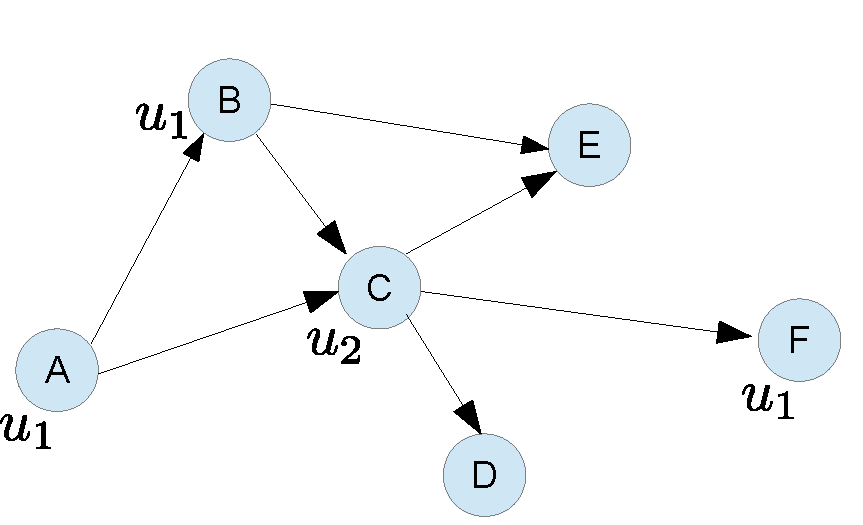
\includegraphics[width=0.33\columnwidth]{previous-articles/adjoint/figs-gen/gen-net}
\par\end{centering}

}\subfloat[\label{fig:gennetb}]{\begin{centering}
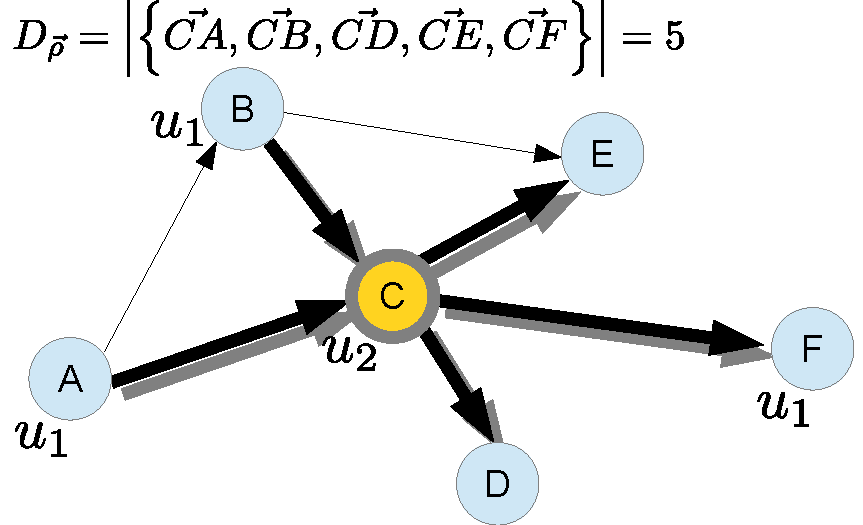
\includegraphics[width=0.33\columnwidth]{previous-articles/adjoint/figs-gen/gen-net-dx}
\par\end{centering}

}\subfloat[\label{fig:gennetc}]{\begin{centering}
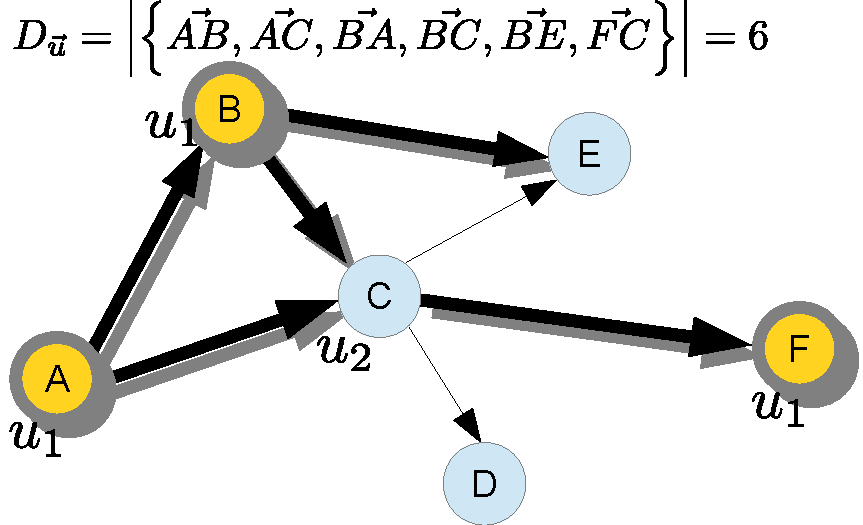
\includegraphics[width=0.33\columnwidth]{previous-articles/adjoint/figs-gen/gen-net-dv}
\par\end{centering}

}
\par\end{centering}

\caption{Depiction of $D_{\state}$ and $D_{v}$ for an arbitrary graph. Fig.~\ref{fig:genneta}
shows the underlying graphical structure for an arbitrary PDE network.
Some control parameter $\convar_{1}$ has influence over junctions
$A$, $B$, and $F$, while another control parameter $\convar_{2}$
has influence over only junction $C$. Fig.~\ref{fig:gennetb}
depicts the center junction having the largest number of connecting
edges, thus giving $D_{\state}=5$. Fig.~\ref{fig:gennetc} shows
that control parameter $\convar_{1}$ influences three junctions with
sum of junctions degrees equal to six, which is maximal over the other
control parameter $\convar_{2}$. leading to the result $D_{\control}=6$.
Note that in Fig.~\ref{fig:gennetc}, the link going from junction
$A$ to junction $B$ is counted twice: once as an outgoing link $\vec{AB}$
and once as in incoming link $\vec{BA}$.\label{fig:Depicting--and}}
\end{figure}

A graphical depiction of $D_{\state}$ and $D_{\control}$ are given
in Fig.~\ref{fig:Depicting--and}. Freeway networks are usually considered to have topologies that are
nearly planar, leading to junctions degrees which typically do not
exceed 3 or 4, regardless of the total number of links. Also, from
the locality argument for control variables in Section~(\ref{sec:State,-control,-and}),
a single control variable's influence over state variables will not
grow with the size of the network. Since the $\DegreeSymbol{\state}$ and
$\DegreeSymbol{\control}$ typically do not grow with $\nlinks\ntime$ or
$\ncontrols\ntime$ for freeway networks, the complexity of evaluating
the gradient for such networks can be considered linear for the adjoint
method.


\subsection{Evaluating the Partial Derivatives\label{sub:Evaluating--and}}

While no assumptions are made about the sparsity of the cost function
$\cost$, the networked-structure of the PDE system and the Godunov
discretization scheme allows us to say more about the structure and
sparsity of $\Hx$ and $\Hu$.


\paragraph{Partial derivative expressions.}

Given that the governing equations require the evaluation of a Riemann
solver at each step, we detail some of the necessary computational
steps in evaluating the $\Hx$ and $\Hu$ matrices. 

If we consider a particular governing equation $\syseq_{\link}^{\tind}\left(\state,\control\right)=0$,
then we may determine the partial term with respect to $\discrete jl\in\state$
by applying the chain rule:

\begin{align}
\pfrac{\syseq_{\link}^{\tind}}{\discrete jl}=\pfrac{\discrete{\link}{\tind}}{\discrete jl}-\pfrac{\discrete{\link}{\tind-1}}{\discrete jl} & +\frac{\Delta t}{L_{i}}f'\left(\RS_{\jdown{\link}}\left(\juncstate{\jdown{\link}}{\tind-1},\junccon{\jdown{\link}}{\tind-1}\right)_{\link}\right)\pfrac{}{\discrete jl}\left(\RS_{\jdown{\link}}\left(\juncstate{\jdown{\link}}{\tind-1},\junccon{\jdown{\link}}{\tind-1}\right)_{\link}\right)\label{eq:dhdufull} \\
& -\frac{\Delta t}{L_{i}}f'\left(\RS_{\jup{\link}}\left(\juncstate{\jup{\link}}{\tind-1},\junccon{\jup{\link}}{\tind-1}\right)_{\link}\right)\pfrac{}{\discrete jl}\left(\RS_{\jup{\link}}\left(\juncstate{\jup{\link}}{\tind-1},\junccon{\jup{\link}}{\tind-1}\right)_{\link}\right)\nonumber                       
\end{align}				
or if we consider the composed Riemann flux solver $\god_{\jn}$ in~\eqref{eq:god-jn}:

\begin{equation}
\pfrac{\syseq_{\link}^{\tind}}{\discrete jl}=\pfrac{\discrete{\link}{\tind}}{\discrete jl}-\pfrac{\discrete{\link}{\tind-1}}{\discrete jl}+\frac{\Delta t}{L_{i}}\left(\pfrac{}{\discrete jl}\left(\god_{\jdown{\link}}\left(\juncstate{\jdown{\link}}{\tind-1},\junccon{\jdown{\link}}{\tind-1}\right)\right)_{\link}-\pfrac{}{\discrete jl}\left(\god_{\jup{\link}}\left(\juncstate{\jup{\link}}{\tind-1},\junccon{\jup{\link}}{\tind-1}\right)\right)_{\link}\right)\label{eq:dhdugod}
\end{equation}


A diagram of the structure of the $\Hx$ matrix is given in Fig.~(\ref{fig:partial-ordering}).
\begin{figure}%
\subfloat[Ordering of the partial derivative terms. Constraints and state variables are clustered first by time, and then by cell index.]{%
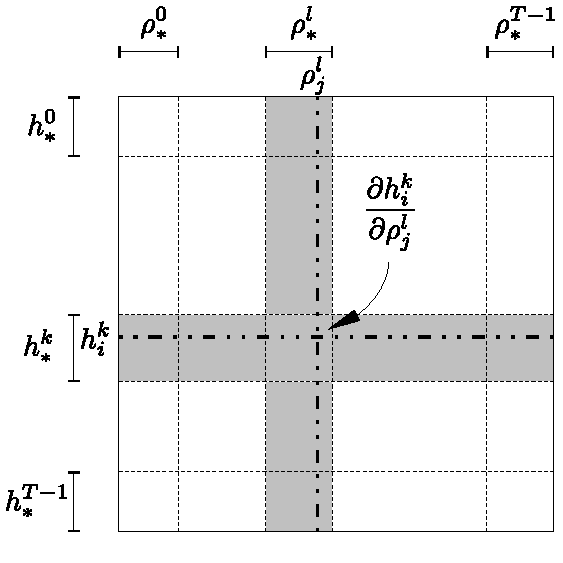
\includegraphics[width=0.43\columnwidth]{previous-articles/adjoint/figs-gen/dstate}%
\label{fig:partial-ordering}%
}\hfill%
\subfloat[Sparsity structure of the $\Hx$ matrix. Besides the diagonal blocks, which are identity matrices, blocks where $l\neq\tind-1$ are zero.]{%
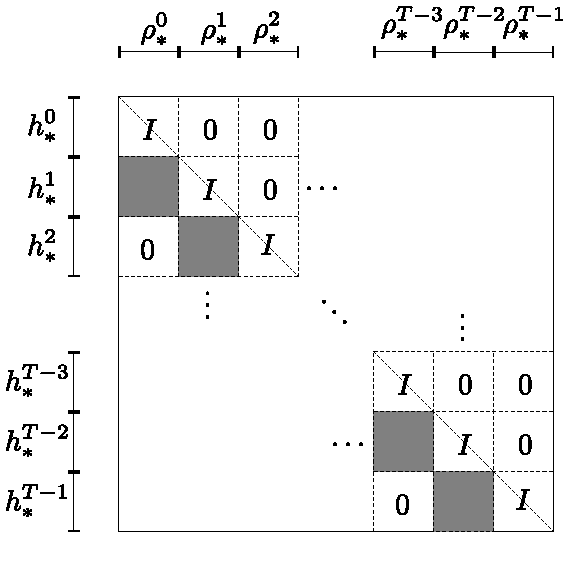
\includegraphics[width=0.43\columnwidth]{previous-articles/adjoint/figs-gen/sparsity-two}%
\label{fig:sparsity-diagram}%
}%
\caption{Structure of the $\Hx$ matrix.}%
\end{figure}
Similarly for $\Hu$, we take a control parameter $\condiscrete jl\in\control$,
and derive the expression:

\begin{align}
\pfrac{\syseq_{\link}^{\tind}}{\condiscrete jl}= & +\frac{\Delta t}{L_{i}}f'\left(\RS_{\jdown{\link}}\left(\juncstate{\jdown{\link}}{\tind-1},\junccon{\jdown{\link}}{\tind-1}\right)_{\link}\right)\pfrac{}{\condiscrete jl}\left(\RS_{\jdown{\link}}\left(\juncstate{\jdown{\link}}{\tind-1},\junccon{\jdown{\link}}{\tind-1}\right)_{\link}\right)\label{eq:dhdvfull} \\
& -\frac{\Delta t}{L_{i}}f'\left(\RS_{\jup{\link}}\left(\juncstate{\jup{\link}}{\tind-1},\junccon{\jup{\link}}{\tind-1}\right)_{\link}\right)\pfrac{}{\condiscrete jl}\left(\RS_{\jup{\link}}\left(\juncstate{\jup{\link}}{\tind-1},\junccon{\jup{\link}}{\tind-1}\right)_{\link}\right)\nonumber                       
\end{align}
or for the composed Godunov junction flux solver $\god_{\jn}$:

\begin{equation}
\pfrac{\syseq_{\link}^{\tind}}{\condiscrete jl}=\frac{\Delta t}{L_{i}}\left(\pfrac{}{\condiscrete jl}\left(\god_{\jdown{\link}}\left(\juncstate{\jdown{\link}}{\tind-1},\junccon{\jdown{\link}}{\tind-1}\right)\right)_{\link}-\pfrac{}{\condiscrete jl}\left(\god_{\jup{\link}}\left(\juncstate{\jup{\link}}{\tind-1},\junccon{\jup{\link}}{\tind-1}\right)\right)_{\link}\right)\label{eqdhdvgod}.
\end{equation}


Analyzing~\eqref{eq:dhdufull}, the only partial terms that are not
trivial to compute are $\pfrac{}{\discrete jl}\left(\RS_{\jdown{\link}}\left(\juncstate{\jdown{\link}}{\tind-1},\junccon{\jdown{\link}}{\tind-1}\right)_{\link}\right)$
and $\pfrac{}{\discrete jl}\left(\RS_{\jup{\link}}\left(\juncstate{\jup{\link}}{\tind-1},\junccon{\jup{\link}}{\tind-1}\right)_{\link}\right)$.
Similarly for~\eqref{eq:dhdvfull}, the only nontrivial terms are
$\pfrac{}{\condiscrete jl}\left(\RS_{\jdown{\link}}\left(\juncstate{\jdown{\link}}{\tind-1},\junccon{\jdown{\link}}{\tind-1}\right)_{\link}\right)$
and $\pfrac{}{\condiscrete jl}\left(\RS_{\jup{\link}}\left(\juncstate{\jup{\link}}{\tind-1},\junccon{\jup{\link}}{\tind-1}\right)_{\link}\right)$.
Once one obtains the solutions to these partial terms, then one can
construct the full $\Hx$ and $\Hu$ matrices and use~\eqref{eq:adjoint}
and~\eqref{eq:adjoint-grad} to obtain the gradient value.

As these expressions are written for a general scalar conservation
law, the only steps in computing the gradient that are specific to
a particular conservation law and Riemann solver are computing the
derivative of the flux function $f$ and the partial derivative terms
just discussed. These expressions are explicitly calculated for the
problem of optimal ramp metering in Section~(\ref{sec:Applications-to-Optimal}).


\subsection{Complexity Analysis of Discrete Adjoint for Sparse Networks}
\label{sub:Complexity-of-solving}

This section demostrates the following proposition:

\begin{prop}
\textup{The total complexity for the adjoint method on a scalar hyperbolic
network of PDEs is }$O(\ntime\left(\DegreeSymbol{\state}\nlinks+\DegreeSymbol{\control}\ncontrols\right))$.\end{prop}

We can show the lower-triangular structure and invertibility of $\Hx$
by examining~\eqref{eq:init-ge} and~\eqref{eq:main-ge}. For $\tind\in\intrange 1{\ntime-1}$,
we have that $\syseq_{\link}^{\tind}$ is only a function of $\discrete{\link}{\tind}$
and of the state variables from the previous time-step $\tind-1$.
Thus, based on our ordering scheme in Section~\ref{sec:State,-control,-and}
of ordering variables by increasing time-step and ordering constraints
by corresponding variable, we know that the diagonal terms of $\Hx$ are
always $1$ and all upper-triangular terms must be zero (since those
terms correspond to constraints with a dependence of \emph{future}
values). These two conditions demonstrate both that $\Hx$ is lower-triangular
and is invertible due to the ones along the diagonal.

Additionally, if we consider taking partial derivatives with respect
to the variable $\discrete jl$, then we can deduce from Equation~\eqref{eq:main-ge}
that all partial terms will be zero except for the diagonal term,
and those terms involving constraints at time $j+1$ with links connecting
to the downstream and upstream junctions $\jdown j$ and $\jup j$
respectively. To summarize, $\Hx$ matrices for systems described
in Section~\ref{sec:State,-control,-and} will be square, invertible,
lower-triangular and each column will have a maximum cardinality equal
to $\DegreeSymbol{\state}$ in~\eqref{eq:dx}. The sparsity structure of
$\Hx$ is depicted in Fig.~\ref{fig:sparsity-diagram}.

Using the same line of argument for the maximum cardinality of $\Hx$,
we can bound the maximum cardinality of each column of $\Hu$. Taking
a single control variable $\condiscrete jl$, the variable can only
appear in the constraints at time-step $j+1$ that correspond to a link
that connects to a junction $\jn$ such that $\condiscrete jl\in\junccon{\jn}{l+1}$.
These conditions give us the expression for $\DegreeSymbol{\control}$ in~\eqref{eq:dv},
or the maximum cardinality over all columns in $\Hu$.

If we only consider the lower triangular form of $\Hx$, then the
complexity of solving for the gradient using the forward system is
$O(\left(\nlinks\ntime\right)^{2}\ncontrols\ntime)$, where the dominating
term comes from solving~\eqref{eq:j-v}, which requires the solution
of $\ncontrols\ntime$ separate $\nlinks\ntime\times\nlinks\ntime$
lower-triangular systems. The lower-triangular system allows for forward
substitution, which can be solved in $O(\left(\nlinks\ntime\right)^{2})$
steps, giving the overall complexity $O(\left(\nlinks\ntime\right)^{2}\ncontrols\ntime)$.
The complexity of computing the gradient via the adjoint method is
$O(\left(\nlinks\ntime\right)^{2}+\left(\nlinks\ntime\right)\left(\ncontrols\ntime\right))$,
which is certainly more efficient than the forward-method, as long
as $\ncontrols\ntime>1$. The efficiency is gained by considering
that~\eqref{eq:adjoint} only requires the solution of a single $\nlinks\ntime\times\nlinks\ntime$
\emph{upper}-triangular system (via backward-substitution), followed
by the multiplication of $\lambda^{T}H_{v}$, an $\nlinks\ntime\times\nlinks\ntime$
and an $\nlinks\ntime\times\ncontrols\ntime$ matrix in~\eqref{eq:adjoint-grad},
with a complexity of $O(\left(\nlinks\ntime\right)^{2}+\left(\nlinks\ntime\right)\left(\ncontrols\ntime\right))$.

For the adjoint method, this complexity can be improved upon by considering
the sparsity of the $\Hx$ and $\Hu$ matrices, as detailed in Section~\ref{sub:Complexity-of-solving}.
For the backward-substitution step, each entry in the $\lambda$ vector
is solved by \emph{at most} $\DegreeSymbol{\state}$ multiplications, and
thus the complexity of solving~\eqref{eq:adjoint} is reduced to
$O(\DegreeSymbol{\state}\nlinks\ntime)$. Similarly, for the matrix multiplication
of $\lambda^{T}H_{v}$, while $\lambda$ is not necessarily sparse,
we know that each entry in the resulting vector requires at most $\DegreeSymbol{\control}$
multiplications, giving a complexity of $O(\DegreeSymbol{\control}\ncontrols\ntime)$. Furthermore, if a sparse implementation of the $\Hx$ and $\Hu$ matrices are used, then memory usage will also scale linearly with the number of state and control variables.


\section{Adjoint-based Model Predictive Control for Coordinated, Predictive Ramp Metering}

\paragraph{Problem Statement}

Including the initial conditions as specified in~\eqref{eq:init-ge}
with~\eqref{eq:rho-update} and~\eqref{eq:ramp-eqn} gives
a complete description of the system $\sys\left(\state,\control\right)=0$,
$\state\in\mathbb{R}^{2\nlinks}$, $\control\in\mathbb{R}$, where:

\begin{eqnarray*}
\state_{2\nlinks\tind+\link}\defeq & \densitydiscrete{\link}{\tind} & 1\le i\le2\nlinks,0\le k\le T-1\\
\control_{\nlinks\tind+\link}\defeq & \ramp_{2\link}^{\tind} & 1\le i\le\nlinks,0\le k\le T-1
\end{eqnarray*}


The objective of the control is to minimize the \emph{total travel
time }on the network, expressed by the cost function $\cost$:

\[
\cost\left(\state,\control\right)=\Delta t\sum_{k=1}^{T}\sum_{i=1}^{2\nlinks}L_{i}\densitydiscrete{\link}{\tind}.
\]


The optimal coordinated ramp-metering problem can be formulated as
an optimization problem with PDE-network constraints:

\begin{eqnarray}
\min_{\control} & \cost\left(\state,\control\right)\label{eq:full}\\
\text{subject to:} & \sys\left(\state,\control\right) & =0\nonumber \\
& 0\le\convar\le1 & \forall\convar\in\control  \label{eq:box}
\end{eqnarray}

Standard methods exist for the handling of geometric constraints on $\mathbf{u}$ in descent methods (such as box constraints in Equation~\eqref{eq:box}), such as projection methods~\cite{d2010modeling} and barrier methods~\cite{Fiacco1990Nonlinear,Boyd2010b,Bayen2006}.

\subsection{Partial Derivative Calculations for Ramp Metering}
\label{sec:Applications-to-Optimal}

To use the adjoint method as described in Section~\ref{sec:discrete-adjoint-method},
we need to compute the partial derivative matrices $\Hx$, $\Hu$,
$\tilde{C}_{\state}$ and $\tilde{C}_{\control}$. Computing the partial
derivatives with respect to the cost function is straight forward:

\begin{eqnarray*}
\pfrac{\tilde{\cost}}{\discrete{\link}{\tind}}= & \Delta tL_{i} & 1\le i\le2\nlinks,0\le k\le T-1\\
\pfrac{\tilde{\cost}}{\ramp_{2\link}^{\tind}}= & \barrierTerm\left(\frac{1}{1-\ramp_{2\link}^{\tind}}-\frac{1}{\ramp_{2\link}^{\tind}}\right) & 1\le i\le\nlinks,0\le k\le T-1
\end{eqnarray*}


To compute the partial derivatives of $\sys$, we follow the procedure
in Section~\ref{sub:Evaluating--and}. For an upstream junction
$\jup{2\link}\in\jns$ and time-step $k\in\intrange 1{\ntime-1}$,
we only need to compute the partial derivatives of the flux solver
$\god_{\jup{2\link}}\left(\juncstate{\jup{2\link}}{\tind},\ramp_{2\link-1}^{\tind}\right)_{\text{}}$
with respect to the adjacent state variables $\juncstate{\jn_{\link}}{\tind}$
and ramp metering control $\ramp_{\link}^{\tind}$. We calculate the
partial derivatives of the functions in~\eqref{eq:first-ramp}-\eqref{eq:last-ramp}
with respect to either a state or control variable$s\in\state\cup\control$:

\begin{eqnarray*}
\pfrac{\demand_{2\left(\link-1\right)}^{\tind}}s & = & \begin{cases}
\ffspeed_{2\left(i-1\right)} & s=\densitydiscrete{2\left(\link-1\right)}{\tind},\ffspeed_{i}\densitydiscrete{2\left(\link-1\right)}{\tind}\le F_{2\left(i-1\right)}^{\max}\\
0 & \text{otherwise}
\end{cases}\\
\pfrac{\supply_{2\link}^{\tind}}s & = & \begin{cases}
-\congspeed_{2i} & s=\densitydiscrete{2\link}{\tind},\congspeed_{2i}\left(\density_{2i}^{\max}-\densitydiscrete{2\link}{\tind}\right)\le F_{2i}^{\max}\\
0 & \text{otherwise}
\end{cases}\\
\pfrac ds & = & \begin{cases}
\ramp_{2\link-1}^{\tind} & s=\densitydiscrete{2\link-1}{\tind},\densitydiscrete{2\link-1}{\tind}\le F_{2\link-1}^{\max}\\
\min\left(\densitydiscrete{2\link-1}{\tind},F_{2i-1}^{\max}\right) & s=\ramp_{2\link-1}^{\tind}\\
0 & \text{otherwise}
\end{cases}\\
\pfrac{}s\fin{2\link}{\tind} & = & \begin{cases}
\splitratio_{2\left(\link-1\right)}^{\tind}\pfrac{\demand_{2\left(\link-1\right)}^{\tind}}s+\pfrac{\rampDemand_{2\left(\link-1\right)}^{\tind}}s & \splitratio_{2\left(\link-1\right)}^{\tind}\demand_{2\left(\link-1\right)}^{\tind}+\rampDemand_{2\link-1}^{\tind}\le\supply_{2\link}^{\tind}\\
\pfrac{\supply_{2\link}^{\tind}}s & \text{otherwise}
\end{cases}\\
\pfrac{}s\fout{2\left(\link-1\right)}{} & = & \begin{cases}
\pfrac{\demand_{2\left(\link-1\right)}^{\tind}}s & \frac{\fin{2\link}{\tind}p_{2(\link-1)}}{1+p_{2(\link-1)}}\ge\frac{\demand_{2\left(\link-1\right)}^{\tind}}{\splitratio_{2\left(\link-1\right)}^{\tind}}\\
\frac{1}{\splitratio_{2\left(\link-1\right)}^{\tind}}\left(\pfrac{}s\fin{2\link}{\tind}-\pfrac{\rampDemand_{2\link-1}^{\tind}}s\right) & \frac{\fin{2\link}{\tind}}{1+p_{2(\link-1)}}\ge\rampDemand_{2\left(\link-1\right)}^{\tind}\\
\frac{p_{2(\link-1)}}{\splitratio_{2\left(\link-1\right)}^{\tind}\left(1+p_{2(\link-1)}\right)}\pfrac{}s\fin{2\link}{\tind} & \text{otherwise}
\end{cases}\\
\pfrac{}s\fout{2\link-1}{} & = & \pfrac{}s\fin{2\link}{\tind}-\splitratio_{2\left(\link-1\right)}^{\tind}\pfrac{}s\fout{2\left(\link-1\right)}{}
\end{eqnarray*}


These expressions fully specify the partial derivative values needed
in~\eqref{eq:dhdugod} and~\eqref{eqdhdvgod}. Thus we can construct
the $\Hx$ and $\Hu$ matrices. With these matrices and $\Jx$ and
$\Ju$, we can solve for the adjoint variable $\lambda\in\mathbb{R}^{2\nlinks\ntime}$
in~\eqref{eq:adjoint} and substitute its value into~\eqref{eq:adjoint-grad}
to obtain the gradient of the cost function $\cost$ with respect
to the control parameter $\control$.

\subsection{Model Predictive Control Overview}
\label{sec:model-predictive-control-overview-adjoint-section}

There are a number of underlying assumptions that permit finite-horizon optimal control techniques to be useful.

\begin{itemize}
	\item The mathematical dynamics accurately models the actual physical system being controlled.
	\item The current state of the system is known.
	\item The future state of the system can be accurately predicted as a function of the applied control.
\end{itemize}

Under an idealized simulation, these conditions are met by assuming perfect knowledge of initial and boundary conditions, and validating performance against using forward simulation identical to the controller's assumed model. In application, the above conditions will not be met exactly due to model inaccuracy, sensor noise, and prediction error. Thus, when applying control policies generated from optimal control procedures in noisy environments, one would expect the future physical state to diverge from that predicted from the controller's model, and thus a degradation in the performance of the controller.

This stems from optimal control being an \emph{open loop} control method, where the error in the state estimation is not observed as the physical system evolves. Alternatively, \emph{closed loop} controllers~\cite{Papageorgiou1991,Papamichail} incorporate the state estimation at frequent intervals (e.g. less than one minute for freeway systems), and choose a control policy which is optimal for only the \emph{next} time-step. Such schemes are also referred to as \emph{reactive} schemes, which react to real-time conditions rather than attempt to anticipate future road conditions (predictive schemes).

\begin{figure}[htbp]
	\centering
	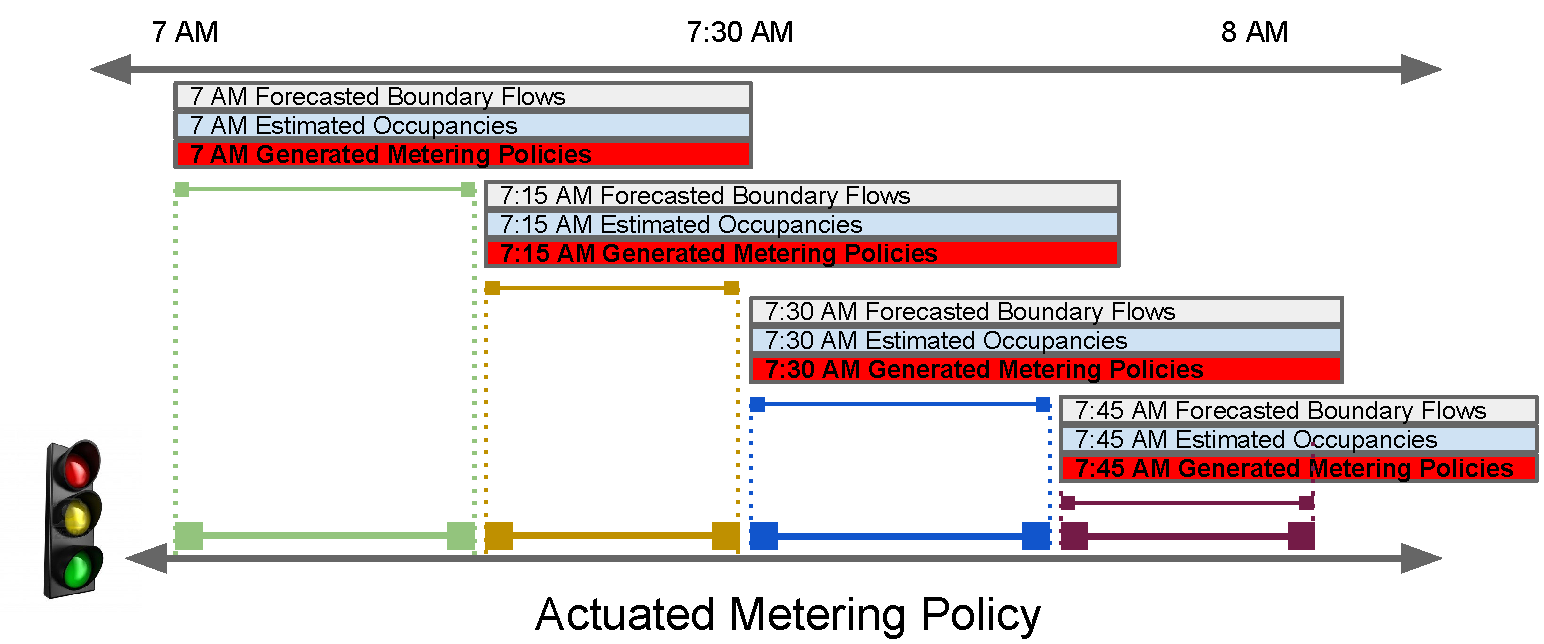
\includegraphics[width=\textwidth]{diagrams/mpc}
	\caption[Diagram of rolling-horizon MPC.]{Diagram of rolling-horizon MPC. At 15 minute intervals ($T_{\text{update}} =15$ minutes), the MPC controller requires an estimate of the current traffic (i.e. initial conditions) as well as predictions over the next 30 minutes ($T_{\text{horizon}} = 30$ minutes) for the future vehicle demands on the on ramps (i.e. boundary conditions).
	}
	\label{fig:mpc-overview}
\end{figure}

\emph{Model predictive control} (MPC) is a control technique which leverages the predictive benefits of optimal control approaches without the drawbacks of open loop control. At time instances occurring with an update period $T_{\text{update}}$, the MPC controller constructs an optimal control problem for the time period between the current time $t$ and some future time $t + T_{\text{horizon}}$, where $T_{\text{horizon}}$ is typically much larger than $T_{\text{update}}$ in order to properly leverage the predictive nature of optimal control. A new control policy is produced for the time period of the current optimal control problem, and the new control policy is then applied to the physical system. After $T_\text{update}$ time has elapsed, an updated control policy will be generated which leverages the newest available initial and boundary conditions. Given that $T_\text{update} < T_\text{horizon}$, the updated policy will be generated before the previous policy is completely applied, at which point the old control policy is discarded in favor of the new policy.


This process is summarized in Figure~\ref{fig:mpc-overview}. An MPC-based controller was implemented within the Connected Corridors system, leveraging the adjoint framework inside the optimal control problem. Numerical results with respect to adjoint control are given in Sections~\ref{sec:numerical-results-adjoint} and~\ref{sec:numerical_results-admm}.


\subsection{Numerical Results}
\label{sec:numerical-results-adjoint}

To demonstrate the effectiveness of using the adjoint ramp metering
method to compute gradients, we implemented the algorithm on practical scenarios with field experimental data.
The algorithm can then be used as a gradient computation subroutine
inside any descent-method optimization solver that takes advantage
of first-order gradient information. Our implementation makes use
of the open-source \emph{IpOpt} solver~\cite{Andreas2005}, an interior point, nonlinear program optimizer. To serve
as comparisons, two other case scenarios were run:
\begin{enumerate}
\item No control: the metering rate is set to 1 on all on-ramps at all times.
\item Alinea~\cite{Papageorgiou1991Alinea}: a well-adopted, feedback-based ramp metering
algorithm commonly used in the practitioner's community. Alinea is computationally efficient and decentralized,
making it a popular choice for large networks, but does not take estimated
boundary flow data as input. Since Alinea has a number of tuning parameters,
we perform a \emph{modified} grid-search technique over the different
parameters that scales linearly with the number of on-ramps, and select
the best-performing parameters, in order to be fair to this framework. A \emph{full} grid-search approach
scales exponentially with the number of on-ramps, rendering it infeasible
for moderate-size freeway networks.
\end{enumerate}
All simulations were run on a 2012 commercial laptop with 8 GB of RAM and a dual-core 1.8 GHz Intel Core i5 processor.

\begin{note} To demonstrate the reduced running time associated with the adjoint approach, we also implemented a gradient descent using a finite differences approach similar to~\cite{Frejo2011,Ramon2013}, which requires an $O(\ntime^2\nlinks\ncontrols)$ computation for each step in gradient descent, but it proved to be computationally infeasible for even small, synthetic
networks. Running ramp metering on even a network of 4 links over
6 time-steps for 5 gradient steps took well over 4 minutes,
rendering the method useless for real-time applications. The comparison
of running times of finite differences versus the adjoint method is given in
Fig.~\ref{fig:Running-time-of}. Due to the impractically large running times associated with finite differences, we do not consider the finite differences in further results, which only becomes worse as the problem scales to larger networks and time horizons.
\end{note}
\begin{figure}[h]
\centering%
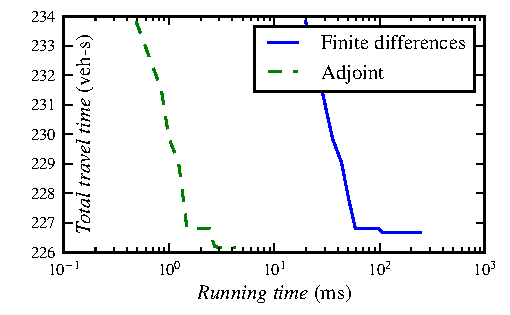
\includegraphics[width=0.5\columnwidth]{previous-articles/adjoint/images/itergrad}%
\caption{Running time of ramp metering algorithm using IpOpt with and without gradient information.
Network consists of 4 links and 6 time-steps with synthetic boundary
flux data. The method using gradient information via the adjoint
method converged well before the completion of the \textit{first} step of the finite differences descent method.
}%
\label{fig:Running-time-of}
\end{figure}



\subsubsection{Implementation of I15S in San Diego\label{sub:Network}}

As input into the optimization problem, we constructed a model of
a 19.4 mile stretch of the I15 South freeway in San Diego,
California between San Marcos and Mira Mesa. The network has $\nlinks=125$ links, and $\ncontrols=9$ on-ramps,
with boundary data specified for $\ntime=1800$ time-steps,
for a time horizon of 120 minutes given $\Delta t=$4 seconds.
The network is shown in Fig.~\ref{fig:Model-of-section}.
\begin{figure}
\centering%
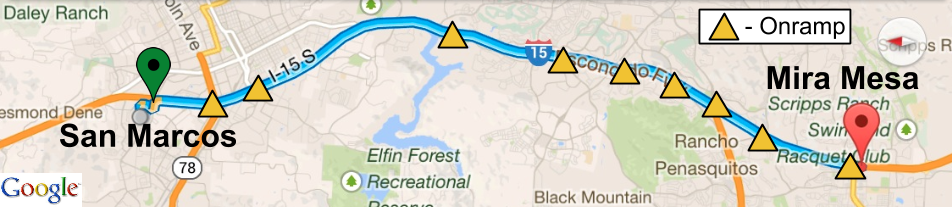
\includegraphics[width=0.65\columnwidth]{previous-articles/adjoint/images/map}%
\caption{Model of section of I15 South in San Diego, California. The freeway section spanning 19.4 miles was split into 125 links with 9 on-ramps.}%
\label{fig:Model-of-section}
\end{figure}


Link length data was obtained using the Scenario Editor software developed
as part of the \textit{Connected Corridors} project, a collaboration between
UC Berkeley and PATH research institute in Berkeley, California.
Fundamental diagram parameters, split ratios, and boundary data were
also obtained using calibration techniques developed by Connected
Corridors. Densities resulting in free-flow speeds were chosen as
initial conditions on the mainline and on-ramps. The data used in calibration
was taken from PeMS sensor data~\cite{Chen2003} during a morning rush hour period,
scaled to generate congested conditions. The input data was chosen
to demonstrate the effectiveness of the adjoint ramp metering method
in a real-world setting. A profile of the mainline and on-ramps during
a forward-simulation of the network is shown in Fig.~\ref{fig:Density-and-queue}
under the described boundary conditions.
\begin{figure}
\subfloat[Density profile. The units are the ratio of a link's vehicle density
to a link's jam density.\label{fig:Density-profile.}]{%
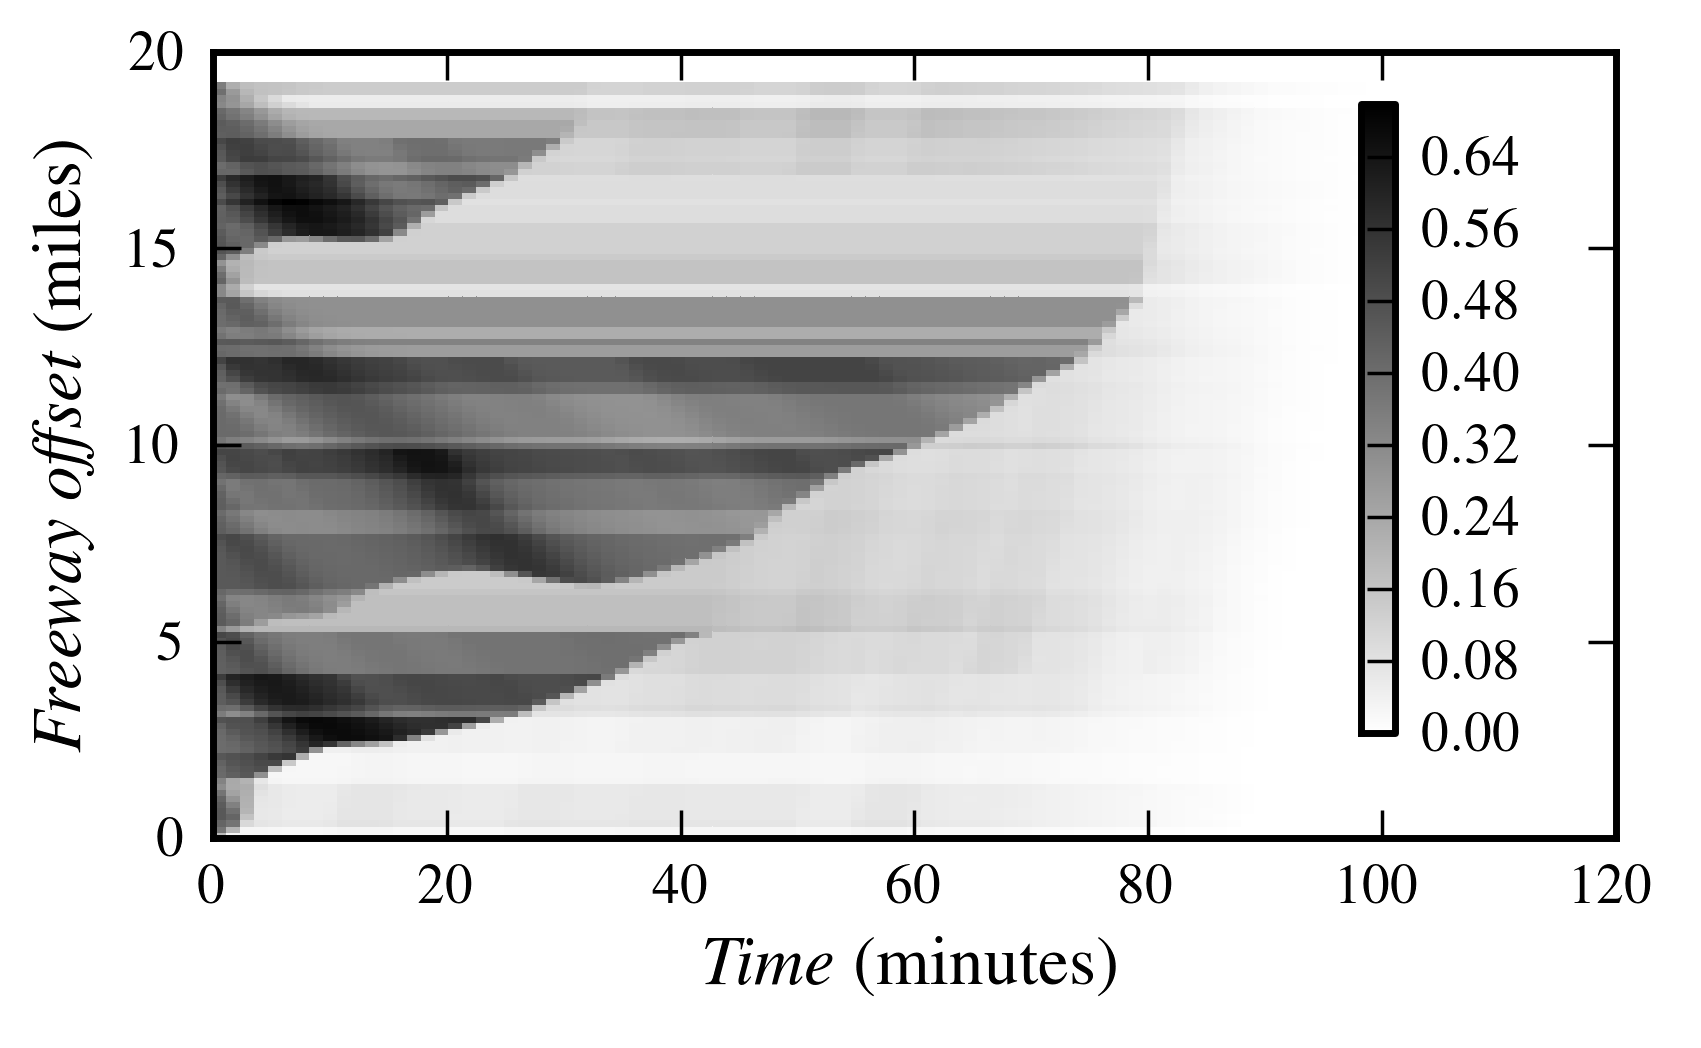
\includegraphics[width=0.45\columnwidth]{previous-articles/adjoint/images/ncdensity}%
}\hfill{}%
\subfloat[On-ramp queue profile in units of vehicles.\label{fig:Density-profile.-2}]{%
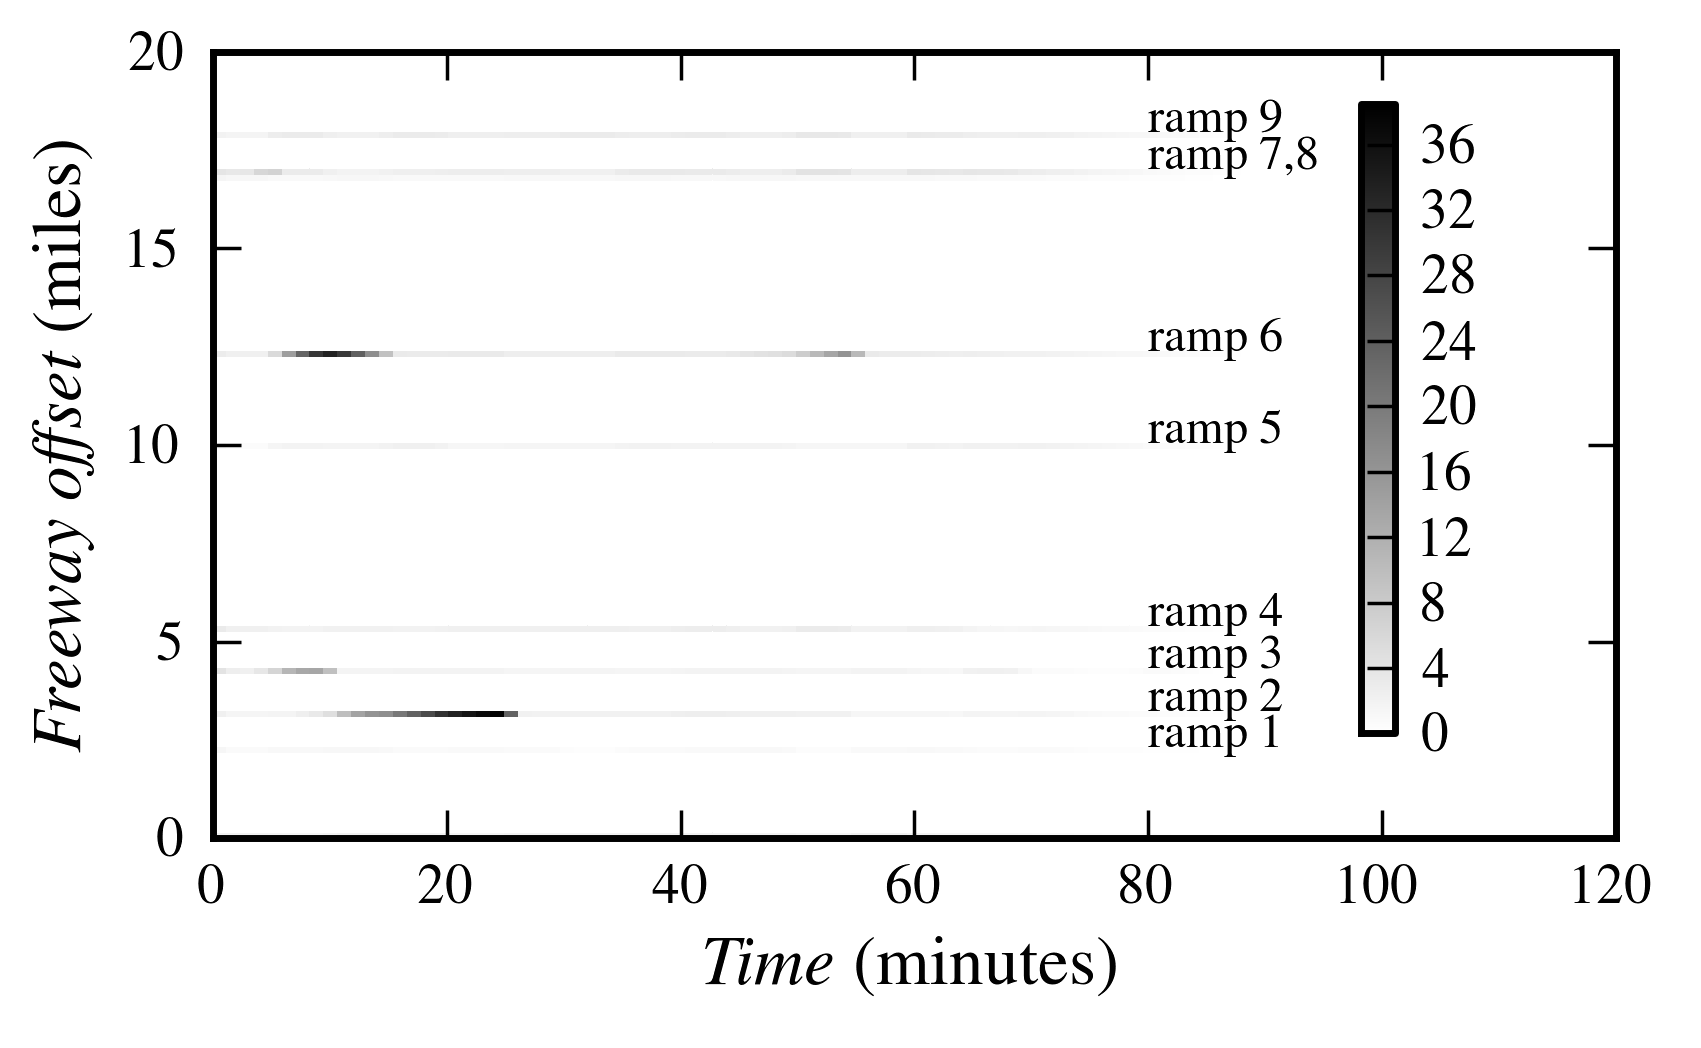
\includegraphics[width=0.45\columnwidth]{previous-articles/adjoint/images/ncqueue}%
}%								
\caption{Density and queue profile of no-control freeway simulation. In the
	first 80 minutes, congestion pockets form on the freeway and queues
	form on the on-ramps, then eventually clear out before 120 minutes.\label{fig:Density-and-queue}}
\end{figure}						
						
\subsubsection{Finite-Horizon Optimal Control\label{sub:Finite-horizon-optimal-control}}
						
						
\paragraph{Experimental Setup.}
						
The adjoint ramp metering algorithm is compared to the reactive Alinea
scheme, for which we assume that perfect boundary conditions and initial conditions
are available. The metric we use to compare the different strategies is \emph{reduced-congestion} percentage, $\bar{c} \in \left(-\infty,100\right]$, which we define as:
\[
\bar{c} = 100 \left(1 - \frac{c_\text{c}}{c_{\text{nc}}}\right)
\]where $c_\text{c}, c_{\text{nc}} \in \mathbb{R}_+$ are the \emph{congestion} resulting from the \emph{control} and \emph{no-control} scenarios, respectively. We use the metric for congestion as defined in~\cite{Skabardonis2003}; for a given section of road $S$ and time horizon $T$, the congestion is given as
\[
c\left(S,T\right) = \sum_{\left(s\in S, \tau\in T\right)} \max \left[\text{TTT}\left(s,\tau\right) - \frac{\text{VMT}\left(s, \tau\right)}{v_s}, 0\right]
\] where $v_s$ is the free-flow velocity, $\text{VMT}$ is total vehicle miles traveled, and $\text{TTT}$ is total travel time over the link $s$ and time-step $\tau$. Since it is infeasible to compute the global optimum for all cases, a reduced congestion of 100\% serves as an upper bound on the possible amount of improvement.

\paragraph{Results.}
						
\begin{figure}[h]
\centering%
\subfloat[Density difference profile in units of \emph{change in density} from the control scenario to the no control scenario over the jam density of the link.]{%
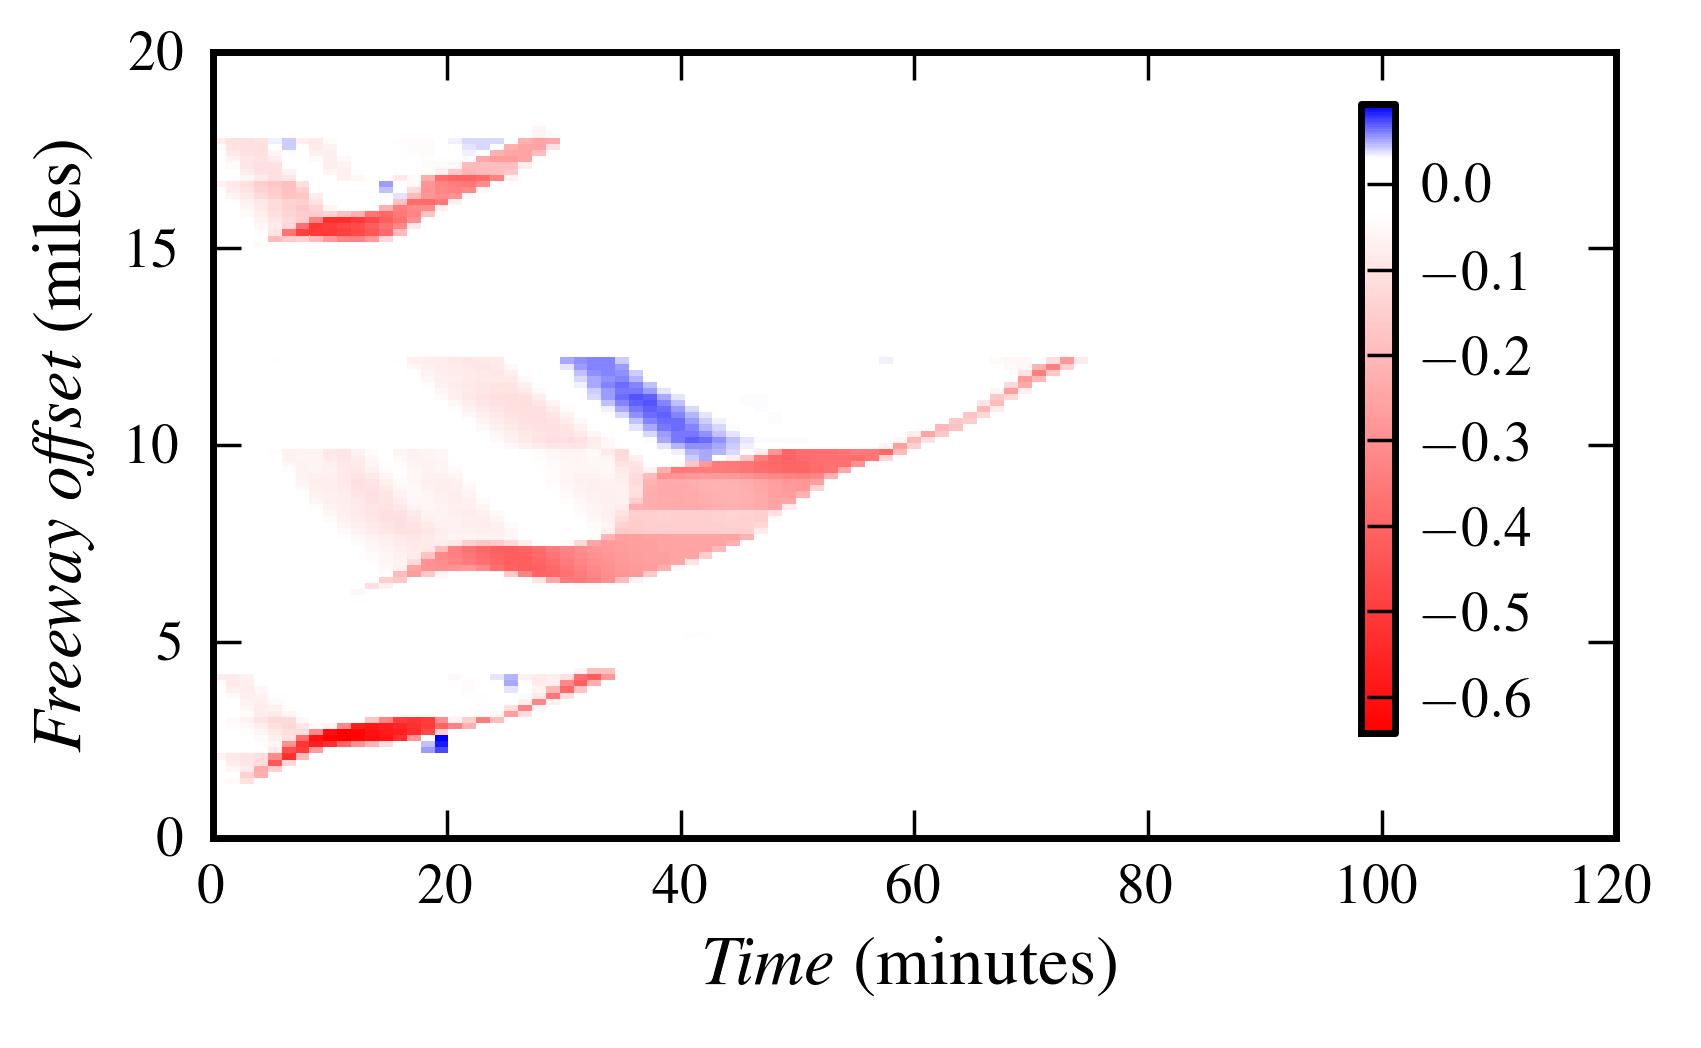
\includegraphics[width=0.45\columnwidth]{previous-articles/adjoint/images/densdiff}%
\label{fig:long-sim-density}%
}\hfill%
\subfloat[Queue difference profile in units of vehicles.]{
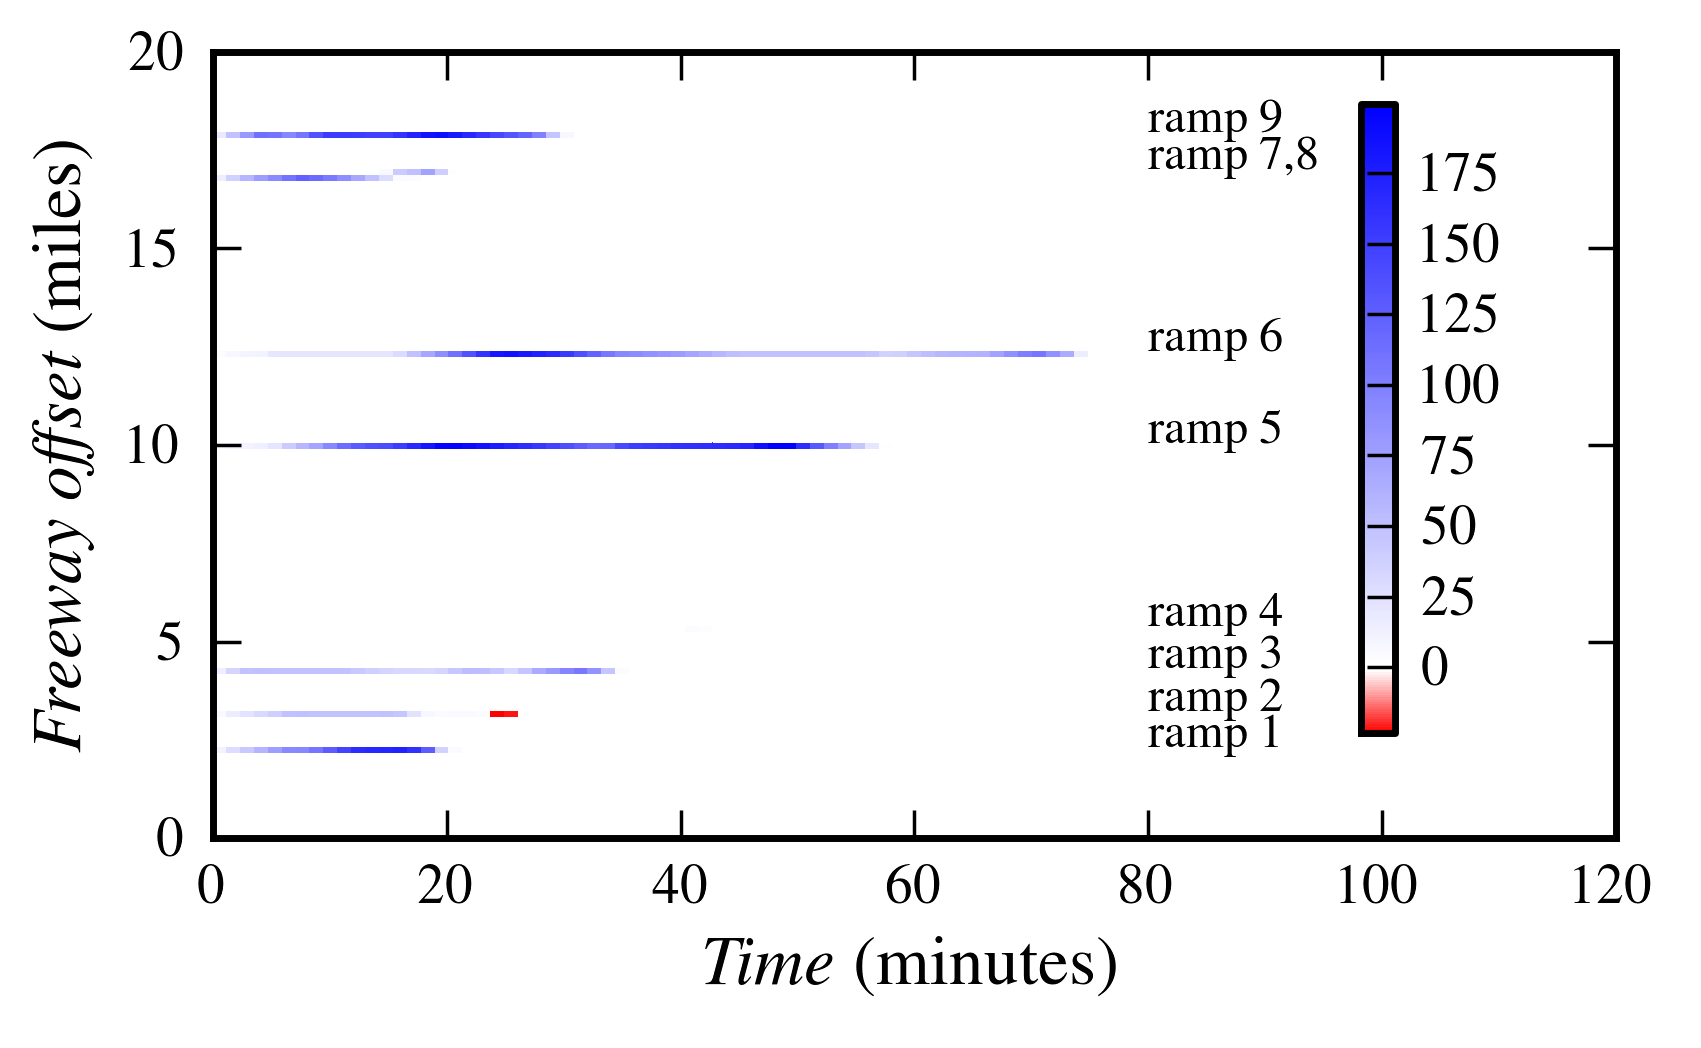
\includegraphics[width=0.45\columnwidth]{previous-articles/adjoint/images/queuediff}%
\label{fig:long-sim-queue}%
}%
\caption{Profile differences for mainline densities and on-ramp queues. Evidenced
	by the mainly negative differences in the mainline densities and the
	mainly positive differences in the on-ramp queue lengths, the adjoint
	ramp metering algorithm effectively limits on-ramp flows in order to
	reduce mainly congestion. \textit{View in color.}\label{fig:long-sim}}
\end{figure}			

Fig.~\ref{fig:long-sim} shows a difference profile for both density and queue lengths between the
no control simulation and the simulation applying the ramp metering
policy generated from the adjoint method. Negative differences in
Figs.~\ref{fig:long-sim-density} and~\ref{fig:long-sim-queue}
indicate where the adjoint method resulted in fewer vehicles for the
specific link and time-step. The adjoint method was successful in
appropriately deciding which ramps should be metered in order to improve
throughput for the mainline.

\begin{figure}[h]
\centering%
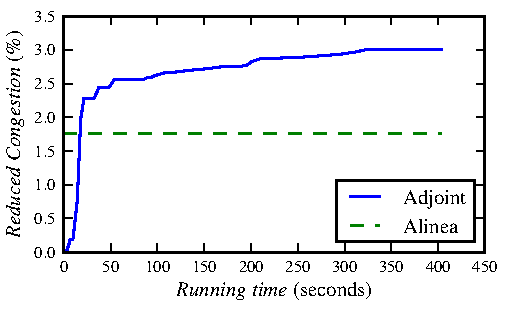
\includegraphics[width=0.45\columnwidth]{previous-articles/adjoint/images/longsim}%
\caption{Reduced congestion versus simulation time for freeway network. The results indicate that the algorithm can run with performance better than Alinea if given an update time of less than a minute.}%
\label{fig:running-time}%
\end{figure}
								
Running time analysis shows that the adjoint method can produce beneficial
results in real-time applications. Fig.~\ref{fig:running-time} details the improvement of the adjoint method as a function of the overall running time of the algorithm. After just a few gradient steps, the
adjoint method outperforms the Alinea method. Given that the time
horizon of two hours is longer than the period of time one can expect
reasonably accurate boundary flow estimates, more practical simulations
with shorter time horizons should permit more gradient steps in a
real-time setting.
								
While the adjoint method leads to queues with a considerable number of cars in some on-ramps, this can be addressed by introducing barrier terms into the cost function that limit the
maximum queue length. The Alinea method tested for the I15 network
had no prescribed maximum queue lengths as well, but was not able
to produce significant improvements in total travel time reduction, while the adjoint method was
more successful.
								
								
\subsubsection{Model Predictive Control\label{sub:Model-predictive-control}}
								
To study the performance of the algorithm under noisy input data,
we embed both our adjoint ramp metering algorithm and the Alinea algorithm
inside of a \emph{model predictive control} (MPC) loop.
								
								
\paragraph{Experimental Setup.}
								
The MPC loop begins at a time $t$ by estimating the initial conditions
of the traffic on the freeway network and the predicted boundary fluxes
over a certain time horizon $T_{h}$. These values are noisy, as exact
estimation of these parameters is not possible on real freeway networks.
The estimated conditions are then passed to the ramp metering algorithm
to compute an optimal control policy over the $T_{h}$ time period.
The system is then forward-simulated over an update period of $T_{u}\le T_{h}$,
using the exact initial conditions and boundary conditions, as opposed
to the noisy data used to compute control parameters. The state of
the system and boundary conditions at $t+T_{u}$ are then estimated
(with noise) and the process is repeated.
								
A non-negative\emph{ noise factor}, $\noiseFactor \in \R_+$, is used to study how the adjoint
method and Alinea perform as the quality of estimated data decreases. If $\discrete{}{}$ is the actual density for a cell and time-step, then the density $\bar{\discrete{}{}}$ passed to the control schemes is given by:
\[
\bar{\discrete{}{}}=\discrete{}{}\cdot \left(1+\noiseFactor\cdot R\right)
\]
where $R$ is a uniformly distributed random variable with mean $0$
and domain $\left[-0.5,0.5\right]$. The noise factor was applied
to both initial and boundary conditions.
								
Two different experiments were conducted:
\begin{enumerate}
	\item \textbf{Real-time I15 South}: MPC is run for the I15 South network
	with $T_{h}=80$ minutes and $T_{u}=26$ minutes. A noise factor of
	2\% was chosen for the initial and boundary conditions. The number
	of iterations was chosen in order to ensure that each MPC iteration
	finished in the predetermined update time $T_{u}$.
	\item \textbf{Noise Robustness}: MPC is for over a synthetic network with
	length 12 miles and boundary conditions over 75 minutes. The experiments
	are run over a profile of noise factors between 1\% and 8000\%.
\end{enumerate}
								
\paragraph{Results.}
								
% \subparagraph{Real-Time I15 South.}
\textbf{Real-Time I15 South.} The results are summarized in Fig.~\ref{fig:MPC-performance-on}.
The adjoint method applied once to the entire horizon with perfect
boundary and initial condition information serves as a baseline performance
for the other simulations, which had noisy input data and limited
knowledge of predicted boundary conditions. The adjoint method still
performs well under the more realistic conditions of the MPC loop
with noise, resulting in 2\% reduced congestion or 40 car-hours in relation to no control, as compared to the 3\% reduced (60 car-hours) congestion achieved by the adjoint method with no noise and full time horizon ($T_h=T$). In comparison, the Alinea method was only able to achieve 1.5\% reduced congestion (30 car-hours) for both the noisy and no-noise scenarios. The results indicate
that, under a realistic assumption of a 2\% noise factor in the sensor
information, the algorithm's ability to consider boundary conditions results in an improvement upon strictly reactive policies,
such as Alinea.
								
\begin{figure}
	\subfloat[Reduced congestion.\label{fig:MPC-performance-on}]{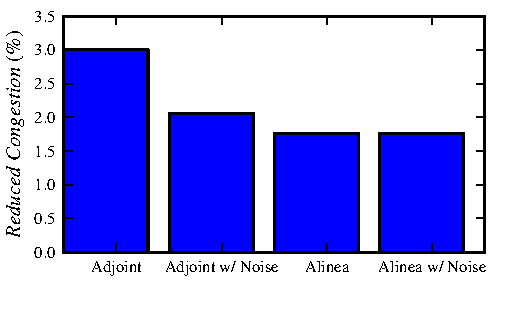
\includegraphics[width=0.45\columnwidth]{previous-articles/adjoint/images/longmpc}
		}\hfill{}\subfloat[Reduced congestion with increasing sensor noise for network with synthetic data.\label{fig:Ramp-metering-performance-1}]{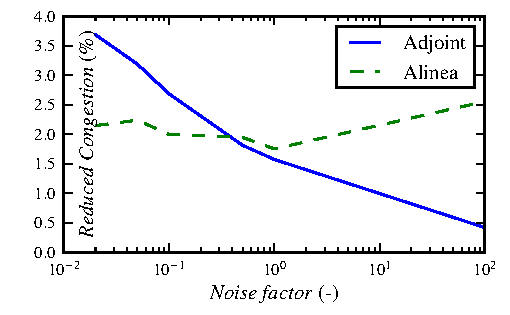
\includegraphics[width=0.45\columnwidth]{previous-articles/adjoint/images/noiseplot}
	}
	\caption{Summary of model predictive control simulations. The results indicate that the adjoint method has superior performance for moderate noise levels on the initial and boundary conditions.}
\end{figure}

% \subparagraph{Robustness to Noise.}																
\textbf{Robustness to Noise.} Simulation results on the synthetic network with varying levels of
noise are shown in Fig.~\ref{fig:Ramp-metering-performance-1}.
The adjoint method is able to outperform the Alinea method when the
noise level is less than 80\%, a reasonable assumption for data provided
by well-maintained loop detectors. As the initial and boundary condition
data deteriorates, the adjoint method becomes useless. Since Alinea
does not rely on boundary data, it is able to produce improvements,
even with severely noisy data. The results indicate that the adjoint
method will outperform Alinea under reasonable noise levels in the
sensor data.


\subsection{Summary of Key Results}

This section has detailed a simple framework for finite-horizon optimal control 
methods on a network of scalar conservation laws derived from first 
discretizing the network via the Godunov method, then applying the discrete 
adjoint to this system. To tailor the framework to a specific application, one 
need only provide the partial derivatives of the Riemann solver at a network 
junction as well as the partial derivatives of the objective. Furthermore, we 
show that for this class of problems, the sparsity pattern allows the problem 
to be implemented with only linear memory and linear computational complexity 
with respect to the number of state and control parameters. We demonstrate the 
scalability of the approach by implementing a coordinated ramp metering 
algorithm using the adjoint method and applying the algorithm to the I-15 South 
freeway in California. The algorithm runs in a fraction of real-time 
and produces significant improvements over existing algorithms. The ramp 
metering algorithm has been fully implemented within Connected 
Corridors~\cite{CC} system, a project by UC Berkeley and PATH for integrated 
corridor management, as a component of the traffic simulator module.